% Provenance (never printed): see sources/outline_sources.md (Year 1: vertical structure of
% the atmosphere, lapse rates, potential temperature and static stability; the layered
% ocean, the equation of state of seawater, T-S diagrams and water masses). Exercise and
% problem values in the Book 3 scratch calculator calc/ch26.py; figures from
% figdata/bachelor-1/atmosphere_profile.py (U.S. Standard Atmosphere 1976) and
% seawater_eos.py (EOS-80 and the UNESCO 44 algorithms; WOA23 columns, datasets
% bachelor-1-woa23-* and Book 2's grade-10-woa23-arctic-*).
% Physics owns the hydrostatic relation, the isothermal atmosphere and its scale height,
% the first law, Laplace's relation and Archimedes' thrust (recalled). Book 1 (g8) gave
% the layers and the environmental lapse rate of 6.5 K/km; Book 2 (g10) the dry adiabatic
% rate admitted, stable and unstable air, the mixed layer, thermocline, halocline and
% pycnocline: re-founded here with derivations. The moist adiabat is the Year 2 volume's.
\chapter{वायुमंडल और महासागर की संरचना}\label{ch:b1:fluid-envelopes-structure}

हर दिन दो बार, दुनिया भर के मौसम-केंद्रों पर, एक गुब्बारा एक रेडियोसॉन्ड के साथ छोड़ा जाता है, एक छोटा उपकरण जो ऊपर उठती हवा का दाब, तापमान और आर्द्रता रेडियो से वापस भेजता है; वह लगभग \qty{300}{m} प्रति मिनट चढ़ता है और गुब्बारे के फटने से पहले \qty{35}{km} तक जा सकता है। समुद्र में दूर, एक अनुसंधान जहाज़ उपकरणों और जल-बोतलों के एक ढाँचे को एक केबल से गहराई तक उतारता है, और पूरे रास्ते चालकता, तापमान और गहराई मापता है। दो परिच्छेद, एक हवा का और एक पानी का, इस अध्याय की कच्ची सामग्री हैं। दोनों परिवेश परतदार हैं, और दोनों में परतबंदी घनत्व से तय होती है: हल्का द्रव नीचे के भारी द्रव के ऊपर। कोई परत हल्की है या भारी, यह दिखने से कम स्पष्ट है। अपने नीचे की हवा से ठंडी हवा फिर भी हल्की हो सकती है; अपने ऊपर के पानी से गरम पानी फिर भी भारी हो सकता है। अध्याय वे दो औज़ार बनाता है जो इसे छाँटते हैं: \omterm{def:b1:fluid-envelopes-structure:potential-temperature}{विभव तापमान} और समुद्री जल का अवस्था-समीकरण।
% ledger: nws:radiosonde, nws:radiosonde-def, commons:ctd-rosette

\begin{omfigure}
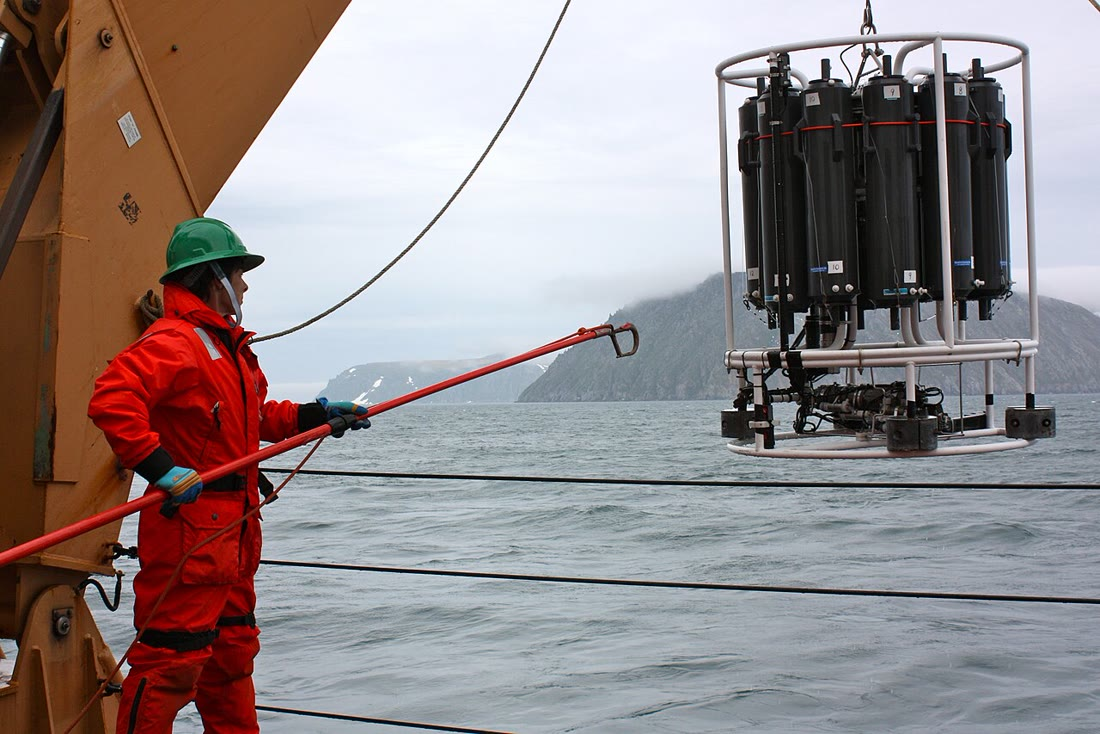
\includegraphics[width=0.62\linewidth]{images/book3/b1-ctd-rosette.jpg}

{\small एक CTD और रोज़ेट को जून 2011 में बेरिंग जलसंधि में जहाज़ पर वापस लाया जा रहा है। ढाँचे के चारों ओर के धूसर बर्तन चुनी गई गहराइयों पर ऊपर आते हुए बंद होते हैं, ताकि पानी का नमूना लिया जा सके; ढाँचे के नीचे के उपकरण चालकता (जिससे लवणता परिकलित होती है), तापमान और गहराई (वास्तव में दाब) लगातार मापते हैं, जब ढाँचा उतारा जाता है। (फ़ोटो: NASA Goddard Space Flight Center, सार्वजनिक डोमेन, विकिमीडिया कॉमन्स के माध्यम से।)}
\label{fig:b1:fluid-envelopes-structure:ctd}
\end{omfigure}
% ledger: commons:ctd-rosette, unesco44:atg-theta

\begin{recall}
भौतिकी खंड विराम में एक तरल के लिए स्थैतिक संबंध $\mathrm dp/\mathrm dz =
-\rho g$ देते हैं; मोलर द्रव्यमान $M$ की एक आदर्श गैस के लिए $p = \rho R
T/M$, और एक समतापीय वायुमंडल में दाब समीकरण $e^{-z/H}$ के साथ गिरता है, जिसमें मापक-ऊँचाई $H = RT/(Mg)$ है। वे एक बंद तंत्र के लिए प्रथम नियम बताते हैं, और आदर्श गैस के लिए उत्क्रमणीय रुद्धोष्म रूपांतरण के साथ लाप्लास का संबंध, $pV^{\gamma} = $ स्थिरांक, जिसमें $\gamma = c_p/c_v$ और प्रति इकाई द्रव्यमान $c_p - c_v
= R/M$। द्रव में डूबे पिंड पर ऊपर की ओर एक उत्प्लावन बल लगता है जो उसके विस्थापित द्रव के भार के बराबर है (आर्किमिडीज़)। पुस्तक~1 ने वायुमंडल की परतों और \omterm{def:b1:fluid-envelopes-structure:standard-atmosphere}{मानक वायुमंडल} के \omterm{def:b1:fluid-envelopes-structure:lapse-rate}{परिवेशी तापह्रास दर} का नामकरण किया था, क्षोभमंडल में \qty{6.5}{\celsius} प्रति किलोमीटर; पुस्तक~2 ने शुष्क रुद्धोष्म दर, \qty{9.8}{\celsius} प्रति किलोमीटर, स्वीकार की, और वायु को उस पिंड के भाग्य के अनुसार स्थायी या अस्थायी कहा जो ऊपर धकेला गया, और महासागर की \omterm{def:b1:fluid-envelopes-structure:ocean-layers}{मिश्रित परत}, \omterm{def:b1:fluid-envelopes-structure:ocean-layers}{ताप-सीमा-परत}, \omterm{def:b1:fluid-envelopes-structure:ocean-layers}{लवण-सीमा-परत} और \omterm{def:b1:fluid-envelopes-structure:ocean-layers}{घनत्व-सीमा-परत} का वर्णन किया। समुद्री जल की लवणता प्रति किलोग्राम लगभग 35 ग्राम घुले लवण के निकट है।
% ledger: ussa76:layers, nws:dalr, nos:salinity
\end{recall}

\section{वायुमंडल की ऊर्ध्वाधर संरचना}\label{sec:b1:fluid-envelopes-structure:atmosphere}

कोई वास्तविक रेडियोसॉन्ड-परिच्छेद अगले के समान नहीं है। उनकी तुलना के लिए एक संदर्भ-परिच्छेद परिपाटी से तय किया जाता है।

\begin{definition}[मानक वायुमंडल]\label{def:b1:fluid-envelopes-structure:standard-atmosphere}
एक \emph{मानक वायुमंडल}\index{मानक वायुमंडल} तापमान, दाब और घनत्व का ऊँचाई के विरुद्ध एक परिच्छेद है जो परिपाटी से तय है: स्थिर मोलर द्रव्यमान का शुष्क वायु, स्थैतिक संतुलन में एक आदर्श गैस, समुद्र-स्तर पर दिए गए मानों के साथ, और एक तापमान जो क्रमिक परतों में ऊँचाई के साथ रैखिक बदलता है। 1976 का मानक वायुमंडल समुद्र-स्तर पर \qty{288.15}{K} और \qty{101325}{Pa} लेता है, $M_0 = \qty{28.9644}{kg.kmol^{-1}}$, $R^* = \qty{8314.32}{J.kmol^{-1}.K^{-1}}$ और $g_0 = \qty{9.80665}{m.s^{-2}}$।
\end{definition}
% ledger: ussa76:sea-level

1976 के मानक में \qty{47}{km} से नीचे चार परतें हैं (\cref{tab:b1:fluid-envelopes-structure:layers})। सबसे निचली, क्षोभमंडल, \qty{6.5}{K} प्रति किलोमीटर ठंडी होती है; उसके ऊपरी सिरे, क्षोभसीमा से, तापमान नौ किलोमीटर तक \qty{216.65}{K} पर रहता है, फिर बढ़ता है। मानक की ऊँचाइयाँ भू-विभव ऊँचाइयाँ हैं, वे ऊँचाइयाँ जो एक स्थिर गुरुत्व $g_0$ वही स्थितिज ऊर्जा देतीं; \qty{32}{km} से नीचे वे ज्यामितीय ऊँचाइयों से \qty{0.6}{\percent} से कम भिन्न हैं (मानक की \qty{11}{km} ऊँचाई \qty{11.02}{km} पर पड़ती है)।
% ledger: ussa76:layers, ussa76:sea-level

\begin{table}[ht]
\centering
\small
\renewcommand{\arraystretch}{1.2}
\begin{tabular}{|l|c|c|c|c|}
\hline
परत & आधार (km) & $\mathrm dT/\mathrm dz$ (K/km) & आधार पर $T$ (K) & आधार पर $p$ (hPa) \\
\hline
1 (क्षोभमंडल) & 0 & $-6.5$ & 288.15 & 1013.25 \\
2 (समतापमंडल) & 11 & 0.0 & 216.65 & 226.32 \\
3 (समतापमंडल) & 20 & $+1.0$ & 216.65 & 54.75 \\
4 (समतापमंडल) & 32 & $+2.8$ & 228.65 & 8.68 \\
\hline
\end{tabular}
\caption{1976 के \omterm{def:b1:fluid-envelopes-structure:standard-atmosphere}{मानक वायुमंडल} की चार निचली परतें। प्रवणताएँ और समुद्र-स्तर के मान परिभाषित मान हैं; आधारों पर तापमान और दाब उनसे \cref{prop:b1:fluid-envelopes-structure:layer-pressure} के साथ परिकलित होते हैं।}
\label{tab:b1:fluid-envelopes-structure:layers}
\end{table}
% ledger: ussa76:layers, ussa76:sea-level (bases computed in figdata/bachelor-1/atmosphere_profile.py)

हर परत में तापमान ऊँचाई का एक रैखिक फलन है, इसलिए स्थैतिक संबंध बंद रूप में समाकलित किया जा सकता है।

\begin{proposition}[एकसमान प्रवणता की परत में दाब]\label{prop:b1:fluid-envelopes-structure:layer-pressure}
शुष्क वायु की एक परत में, जहाँ $T = T_b - L\,(z - z_b)$ है और स्थिर $L \neq 0$ है, दाब
\[
  p = p_b \left(\frac{T}{T_b}\right)^{gM/(RL)},
\]
जहाँ $T_b$ और $p_b$ आधार $z_b$ पर के मान हैं। जब $L = 0$ हो, तो दाब मापक-ऊँचाई $H = RT_b/(Mg)$ के साथ घातांकीय रूप से गिरता है।
\end{proposition}

\begin{proof}
स्थैतिक संबंध और आदर्श गैस देते हैं $\mathrm dp/p = -(gM/R)\,\mathrm
dz/T$। चूँकि $\mathrm dT = -L\,\mathrm dz$ है, यह $\mathrm dp/p =
(gM/(RL))\,\mathrm dT/T$ है, जो $\ln(p/p_b) = (gM/(RL))
\ln(T/T_b)$ तक समाकलित होता है। $L = 0$ के लिए, $T = T_b$ और $\ln(p/p_b) = -(z - z_b)/H$: भौतिकी खंडों का समतापीय वायुमंडल।
\end{proof}

मानक के क्षोभमंडल में, $gM/(RL) = 9.80665 \times 28.9644 /
(8314.32 \times 0.0065) = 5.256$ है, और \qty{11}{km} पर, $T = 216.65$~K: $p = \num{101325} \times (216.65/288.15)^{5.256} = \qty{22632}{Pa}$, समुद्र-स्तर के मान के चौथाई से थोड़ा कम। ऊपर की समतापीय परत में, $H =
8314.32 \times 216.65/(28.9644 \times 9.80665) = \qty{6.34}{km}$, और नौ किलोमीटर ऊपर दाब एक और गुणक $e^{9/6.34} =
4.13$ से गिर गया है, \qty{5475}{Pa} तक। चूँकि किसी स्तर पर दाब उसके ऊपर की हवा का प्रति इकाई क्षेत्रफल भार है, \omterm{def:b1:fluid-envelopes-structure:standard-atmosphere}{मानक वायुमंडल} का आधा द्रव्यमान \qty{5.5}{km} से नीचे और नौ-दसवाँ भाग \qty{16}{km} से नीचे है।
% ledger: ussa76:sea-level, ussa76:layers (values computed in figdata/bachelor-1/atmosphere_profile.py)

\section{तापह्रास दरें और विभव तापमान}\label{sec:b1:fluid-envelopes-structure:lapse}

\begin{definition}[परिवेशी और शुष्क रुद्धोष्म तापह्रास दरें]\label{def:b1:fluid-envelopes-structure:lapse-rate}
\emph{परिवेशी तापह्रास दर}\index{परिवेशी तापह्रास दर} $\Gamma =
-\mathrm dT/\mathrm dz$ है, वह दर जिससे विराम में हवा का तापमान ऊँचाई के साथ घटता है, जैसा एक परिच्छेद उसे मापता है। \emph{शुष्क रुद्धोष्म तापह्रास दर}\index{शुष्क रुद्धोष्म तापह्रास दर} $\Gamma_d$ वह दर है जिससे असंतृप्त वायु के एक पिंड का तापमान घटता है जब पिंड उठाया जाता है।
\end{definition}
% ledger: nws:dalr

जब तापमान ऊँचाई के साथ घटता है तो तापह्रास दर धनात्मक होती है। दोनों दरें भिन्न प्रकृति की हैं: पहली वायुमंडल की स्थिति एक क्षण में बताती है; दूसरी गतिमान हवा के एक टुकड़े का रूपांतरण।

\begin{definition}[वायु-पिंड]\label{def:b1:fluid-envelopes-structure:parcel}
एक \emph{वायु-पिंड}\index{वायु-पिंड} हवा का एक आयतन है जो उसकी गति में अनुसरित किया जाता है, इतना छोटा कि उसका एक ही तापमान और दाब हो और वह अपने चारों ओर की हवा को विचलित न करे, और इतना बड़ा कि अपनी पहचान बनाए रखे: वह द्रव्यमान का आदान-प्रदान नहीं करता, और एक तेज़ विस्थापन के दौरान अपने परिवेश के साथ ऊष्मा का भी नहीं, और उसका दाब हर क्षण आसपास की हवा का दाब होता है।
\end{definition}

\omterm{def:b1:fluid-envelopes-structure:parcel}{वायु-पिंड} एक आदर्शीकरण है, ऊष्मगतिकी के बंद तंत्र की तरह: नीचे के परिणाम वास्तविक हवा के लिए तब तक लागू होते हैं जब तक उसका गतिमान टुकड़ा अपने परिवेश के साथ कम ऊष्मा और कम द्रव्यमान का आदान-प्रदान करता है।

\begin{theorem}[शुष्क रुद्धोष्म तापह्रास दर]\label{thm:b1:fluid-envelopes-structure:dry-adiabatic}
शुष्क हवा का एक पिंड, जिसे रुद्धोष्म और उत्क्रमणीय रूप से लगभग उसी तापमान की विराम हवा के आर-पार उठाया जाता है, इस दर से ठंडा होता है
\[
  \Gamma_d = \frac{g}{c_p},
\]
जहाँ $c_p$ स्थिर दाब पर हवा की विशिष्ट ऊष्मा है। $c_p =
\qty{1004.7}{J.kg^{-1}.K^{-1}}$ के साथ, $\Gamma_d = \qty{9.76}{K.km^{-1}}$।
\end{theorem}

\begin{proof}
पिंड के एक किलोग्राम के लिए, जिसका तापमान $T_p$ और घनत्व $\rho_p$ है, ऊष्मा-विनिमय के बिना एक उत्क्रमणीय रूपांतरण का प्रथम नियम, एन्थैल्पी के साथ लिखा, $c_p\,\mathrm dT_p - \mathrm dp/\rho_p = 0$ है। पिंड का दाब उसके चारों ओर की हवा का है, जो स्थैतिक है: $\mathrm dp = -\rho_e
g\,\mathrm dz$, जहाँ $\rho_e$ परिवेशी हवा का घनत्व है। अतः
\[
  \frac{\mathrm dT_p}{\mathrm dz} = -\frac{g}{c_p}\,\frac{\rho_e}{\rho_p}
  = -\frac{g}{c_p}\,\frac{T_p}{T_e},
\]
चूँकि समान दाब पर एक ही मोलर द्रव्यमान की दो आदर्श गैसों के घनत्व उनके तापमानों के व्युत्क्रम अनुपात में हैं। जब पिंड अपने परिवेश के लगभग तापमान पर है, $T_p/T_e \approx 1$ और $-\mathrm dT_p/\mathrm dz
= g/c_p$। शुष्क हवा के लिए, एक आदर्श द्वि-परमाणुक गैस, $\gamma = 1.4$ है, इसलिए $c_p =
\gamma/(\gamma - 1) \times R/M = 3.5 \times 8314.32/28.9644 =
\qty{1004.7}{J.kg^{-1}.K^{-1}}$, और $\Gamma_d = 9.80665/1004.7 =
\qty{0.00976}{K.m^{-1}}$।
\end{proof}
% ledger: nasa:grc-gamma, ussa76:sea-level, nws:dalr

\qty{280}{K} के निकट, अपने परिवेश से \qty{10}{K} गरम एक पिंड $\Gamma_d \times 290/280$ पर ठंडा होता है, \qty{3.6}{\percent} तेज़; सुधार को आगे नज़रअंदाज़ किया गया है। दर पिंड के दाब या तापमान पर निर्भर नहीं करती, और नीचे डूबता पिंड उसी दर से गरम होता है, जैसा पुस्तक~2 में पहाड़ पर उठती हवा का अनुसरण किया गया था।

उसी समीकरण को स्थैतिक चरण के बिना समाकलित करने पर एक ऐसी राशि मिलती है जिसे पिंड अपने साथ लिए चलता है।

\begin{proposition}[विभव तापमान]\label{prop:b1:fluid-envelopes-structure:theta}
शुष्क हवा के एक उत्क्रमणीय रुद्धोष्म रूपांतरण के साथ,
\[
  \theta = T\left(\frac{p_0}{p}\right)^{\kappa},\qquad \kappa = \frac{R}{Mc_p} =
  \frac{\gamma - 1}{\gamma} = \frac{2}{7},
\]
संदर्भ दाब $p_0$ कुछ भी हो, स्थिर रहता है।
\end{proposition}

\begin{proof}
$c_p\,\mathrm dT = \mathrm dp/\rho$ और $\rho = pM/(RT)$ से, $c_p\,\mathrm dT/T
= (R/M)\,\mathrm dp/p$, इसलिए $\ln T - \kappa \ln p$ स्थिर है, और इसी तरह $T
p^{-\kappa}$; स्थिरांक $p_0^{\kappa}$ से गुणा करने पर $\theta$ मिलता है। यह $T$ और $p$ में लिखा लाप्लास का संबंध है।
\end{proof}

\begin{definition}[विभव तापमान]\label{def:b1:fluid-envelopes-structure:potential-temperature}
शुष्क हवा के एक पिंड का \emph{विभव तापमान}\index{विभव तापमान} $\theta$ वह तापमान है जो उसका होता यदि उसे रुद्धोष्म रूप से संदर्भ दाब $p_0 = \qty{1000}{hPa}$ तक लाया जाता: $\theta = T\,(1000/p)^{2/7}$ जिसमें $p$ हेक्टोपास्कल में और $T$ केल्विन में है।
\end{definition}
% ledger: nws:potential-temperature

\omterm{def:b1:fluid-envelopes-structure:potential-temperature}{विभव तापमान} एक ऐसा लेबल है जिसे शुष्क पिंड उठते या डूबते समय ऊष्मा का आदान-प्रदान किए बिना बनाए रखता है, जैसे जल-पिंड की लवणता। विकिरण से गरम होना, जल के संघनन से, या मिश्रण से उसमें परिवर्तन आता है; बाकी नहीं।

\begin{example}[मानक वायुमंडल का क्षोभसीमा]\label{ex:b1:fluid-envelopes-structure:tropopause}
मानक के सतह पर, $\theta = 288.15 \times (1000/1013.25)^{2/7} =
\qty{287.07}{K}$। क्षोभसीमा पर, $T = \qty{216.65}{K}$ और $p =
\qty{226.32}{hPa}$: $\theta = 216.65 \times (1000/226.32)^{2/7} = 216.65 \times
1.529 = \qty{331.2}{K}$। क्षोभसीमा से रुद्धोष्म रूप से \qty{1000}{hPa} तक नीचे लाई गई हवा \qty{331.2}{K} पर पहुँचती, वही दाब पर लाई गई सतही हवा से \qty{44}{K} गरम। ज़मीन से क्षोभसीमा तक तापमान \qty{71.5}{K} गिरता है, फिर भी \omterm{def:b1:fluid-envelopes-structure:potential-temperature}{विभव तापमान} \qty{44}{K} बढ़ता है।
\end{example}
% ledger: ussa76:layers, nws:potential-temperature (values computed in figdata/bachelor-1/atmosphere_profile.py)

\section{स्थैतिक स्थिरता}\label{sec:b1:fluid-envelopes-structure:stability}

\begin{definition}[स्थैतिक स्थिरता; तापमान-व्युत्क्रमण]\label{def:b1:fluid-envelopes-structure:stability}
परत की विराम में \emph{स्थैतिक स्थिरता}\index{स्थैतिक स्थिरता} एक \omterm{def:b1:fluid-envelopes-structure:parcel}{वायु-पिंड} के एक छोटे ऊर्ध्वाधर विस्थापन पर उसकी प्रतिक्रिया है। परत \emph{स्थायी स्तरीकरण}\index{स्थायी स्तरीकरण} की है यदि विस्थापित पिंड अपने स्तर की ओर वापस धकेला जाता है, \emph{अस्थायी स्तरीकरण}\index{अस्थायी स्तरीकरण} की यदि वह और दूर धकेला जाता है, और \emph{उदासीन स्तरीकरण}\index{उदासीन स्तरीकरण} की यदि उस पर कोई बल नहीं लगता। \emph{तापमान-व्युत्क्रमण}\index{तापमान-व्युत्क्रमण} एक ऐसी परत है जिसमें तापमान ऊँचाई के साथ बढ़ता है।
\end{definition}
% ledger: nws:inversion

\begin{theorem}[स्थैतिक स्थिरता का मानदंड]\label{thm:b1:fluid-envelopes-structure:stability}
तापमान $T$ और \omterm{def:b1:fluid-envelopes-structure:lapse-rate}{परिवेशी तापह्रास दर} $\Gamma$ की विराम में शुष्क वायु की एक परत स्थायी है यदि $\Gamma < \Gamma_d$, उदासीन यदि $\Gamma = \Gamma_d$, और अस्थायी यदि $\Gamma > \Gamma_d$ है; समतुल्य रूप से, वह तभी स्थायी है जब उसका \omterm{def:b1:fluid-envelopes-structure:potential-temperature}{विभव तापमान} ऊँचाई के साथ बढ़े। स्थायी परत में $\delta z$ से थोड़ा विस्थापित एक पिंड अपने स्तर के चारों ओर कोणीय आवृत्ति $N$ पर दोलन करता है, जहाँ
\[
  N^2 = \frac{g}{T}\,(\Gamma_d - \Gamma) = \frac{g}{\theta}\,\frac{\mathrm d\theta}{\mathrm dz}.
\]
\end{theorem}

\begin{proof}
एक पिंड जो अपने स्तर के तापमान $T$ पर है, $\delta z$ से उठाया जाता है। वह $T - \Gamma_d\,\delta z$ पर पहुँचता है, जबकि उसके चारों ओर की हवा $T - \Gamma\,\delta z$ पर है। प्रति इकाई द्रव्यमान, पिंड पर उसका भार और आर्किमिडीज़ का उत्प्लावन लगते हैं, जिससे एक शुद्ध ऊर्ध्वमुखी त्वरण $g\,(\rho_e - \rho_p)/\rho_p = g\,(T_p - T_e)/T_e$ है, दाब बराबर होने से। $\delta z$ में पहली कोटि तक यह है
\[
  \frac{\mathrm d^2 \delta z}{\mathrm dt^2} = -\frac{g}{T}\,(\Gamma_d - \Gamma)\,\delta z = -N^2\,\delta z .
\]
यदि $\Gamma < \Gamma_d$, तो $N^2 > 0$ और पिंड कोणीय आवृत्ति $N$ पर दोलन करता है; यदि $\Gamma > \Gamma_d$ तो विस्थापन घातांकीय रूप से बढ़ता है; यदि $\Gamma = \Gamma_d$ तो कोई बल नहीं लगता। दूसरे रूप के लिए, $\theta = T (p_0/p)^{\kappa}$ का लघुगणकीय अवकलज लीजिए और स्थैतिक संबंध का उपयोग कीजिए:
\[
  \frac{1}{\theta}\frac{\mathrm d\theta}{\mathrm dz} = \frac{1}{T}\frac{\mathrm dT}{\mathrm dz}
  - \frac{\kappa}{p}\frac{\mathrm dp}{\mathrm dz} = -\frac{\Gamma}{T} + \frac{\kappa\,\rho g}{p}
  = -\frac{\Gamma}{T} + \frac{\kappa g M}{RT} = \frac{\Gamma_d - \Gamma}{T},
\]
चूँकि $\kappa M/R = 1/c_p$।
\end{proof}

कोणीय आवृत्ति $N$ को उत्प्लावन आवृत्ति कहते हैं। मानक के पास भू-तल पर, क्षोभमंडल में, $N^2 = (9.80665/288.15) \times (9.761 -
6.5)\times10^{-3} = \qty{1.11e-4}{s^{-2}}$, $N = \qty{0.0105}{s^{-1}}$, और दोलन का आवर्तकाल $2\pi/N$ लगभग \qty{10}{min} है। निचले समतापमंडल में, जहाँ $\Gamma = 0$ है, $N = \qty{0.0210}{s^{-1}}$ है, दुगुना बड़ा, पाँच मिनट का आवर्तकाल। समतापमंडल एक ढक्कन है: वह ऊर्ध्वाधर गति का नीचे के क्षोभमंडल से कहीं अधिक दृढ़ता से प्रतिरोध करता है।
% ledger: ussa76:layers (values computed in figdata/bachelor-1/atmosphere_profile.py)

\begin{omfigure}
\begin{tikzpicture}
\begin{axis}[name=tz, omrecord, width=0.46\linewidth, height=7.2cm, xmin=160, xmax=300,
  ymin=0, ymax=32, xlabel={तापमान (K)}, ylabel={ऊँचाई (km)}, xtick={160,200,...,300},
  ytick={0,5,...,30}]
% figdata/bachelor-1/atmosphere_profile.py; ledger: ussa76:sea-level, ussa76:layers, nasa:grc-gamma
\addplot[omDef, line width=0.9pt] table[x=T_K, y=z_km] {figdata/out/bachelor-1-atmosphere_profile-profile.dat};
\addplot[omThm, dashed, line width=0.7pt] table[x=T_K, y=z_km] {figdata/out/bachelor-1-atmosphere_profile-adiabat.dat};
\addplot[only marks, mark=*, mark size=1.6pt, black] table[x=T_K, y=z_km] {figdata/out/bachelor-1-atmosphere_profile-tropo.dat};

\node[font=\scriptsize, text=omThm, anchor=west, align=left] at (axis cs:163,17.0) {शुष्क रुद्धोष्म\\सतह से};

\node[font=\scriptsize, text=omDef, anchor=west] at (axis cs:252,6.4) {मानक};

\node[font=\scriptsize, anchor=east] at (axis cs:214.5,11.9) {क्षोभसीमा};
\end{axis}
\begin{axis}[at={(tz.east)}, anchor=west, xshift=1.3cm, omrecord, width=0.46\linewidth, height=7.2cm,
  xmin=250, xmax=900, ymin=0, ymax=32, xlabel={विभव तापमान (K)}, ylabel={ऊँचाई (km)},
  xtick={300,500,700,900}, ytick={0,5,...,30}]
\addplot[omDef, line width=0.9pt] table[x=theta_K, y=z_km] {figdata/out/bachelor-1-atmosphere_profile-profile.dat};
\addplot[only marks, mark=*, mark size=1.6pt, black] table[x=theta_K, y=z_km] {figdata/out/bachelor-1-atmosphere_profile-tropo.dat};
\node[font=\scriptsize, anchor=west] at (axis cs:345,10.2) {\num{331} K};
\end{axis}
\end{tikzpicture}

{\small 1976 का \omterm{def:b1:fluid-envelopes-structure:standard-atmosphere}{मानक वायुमंडल} \qty{32}{km} तक। बायीं ओर: तापमान, और वह शुष्क रुद्धोष्म रेखा जिसका सतह से उठाया गया पिंड अनुसरण करेगा (धराशायी)। मानक रुद्धोष्म से धीरे ठंडा होता है, इसलिए वह हर जगह स्थायी है। दायीं ओर: \omterm{def:b1:fluid-envelopes-structure:potential-temperature}{विभव तापमान}, जो पूरे रास्ते ऊँचाई के साथ बढ़ता है, क्षोभमंडल में धीरे और क्षोभसीमा के ऊपर तीव्रता से (बिंदु)।}
\label{fig:b1:fluid-envelopes-structure:theta}
\end{omfigure}
% ledger: ussa76:sea-level, ussa76:layers, nasa:grc-gamma, nws:potential-temperature

ऊँचाई के विरुद्ध तापमान के एक आरेख पर, कसौटी दो ढलानों की तुलना करती है (नीचे का चित्र): पिंड अपने प्रारंभिक बिंदु से गुज़रती शुष्क रुद्धोष्म रेखा का अनुसरण करता है, और प्रश्न यह है कि एक छोटे विस्थापन के बाद वह परिच्छेद के किस ओर पाता है।

\begin{omfigure}
\begin{tikzpicture}[x=0.55cm, y=0.55cm, >={Stealth[length=2mm]}]
\foreach \dx/\envtop/\verdict in {0/-0.8/{स्थायी परत: पिंड नीचे लौटता है}, 9/-3.8/{अस्थायी परत: पिंड और ऊपर उठता है}} {
  \begin{scope}[xshift=\dx cm]
  \draw[->] (0,0) -- (7.2,0) node[below left, font=\scriptsize] {तापमान};
  \draw[->] (0,0) -- (0,6.4) node[above right, font=\scriptsize] {ऊँचाई};
  % sounding (environment): solid; dry adiabat through the starting point P: dashed
  \draw[omDef, line width=0.9pt] (5.0,0.6) -- (5.0+\envtop,5.4);
  \draw[omThm, dashed, line width=0.8pt] (5.0,0.6) -- (2.6,5.4);
  \fill (5.0,0.6) circle (2pt) node[right, font=\scriptsize] {$P$};
  \draw[densely dotted] (0,4.2) node[left, font=\scriptsize] {$z + \delta z$} -- (7,4.2);
  \fill[omThm] (3.2,4.2) circle (1.8pt);
  \fill[omDef] ({5.0+\envtop*3.6/4.8},4.2) circle (1.8pt);
  \node[font=\scriptsize, anchor=north] at (3.6,-0.5) {\verdict};
  \end{scope}
}
\end{tikzpicture}

{\small पार्सल विधि। नीला ठोस: परिच्छेद; लाल धराशायी: $P$ से गुज़रती शुष्क रुद्धोष्म रेखा। एक पिंड $P$ पर अपने चारों ओर की हवा के तापमान पर शुरू होता है और शुष्क रुद्धोष्म रेखा के साथ $z + \delta z$ तक उठाया जाता है (लाल बिंदु); परिच्छेद वहाँ की हवा का तापमान देता है (नीला बिंदु)। बायीं ओर: परिच्छेद रुद्धोष्म से धीरे ठंडा होता है; पिंड अपने परिवेश से ठंडा, इसलिए भारी, पहुँचता है और वापस नीचे बैठता है। दायीं ओर: परिच्छेद रुद्धोष्म से तेज़ी से ठंडा होता है; पिंड गरम पहुँचता है और उठता रहता है।}
\label{fig:b1:fluid-envelopes-structure:parcel}
\end{omfigure}

\begin{method}[परिच्छेद की स्थिरता पढ़ना]\label{met:b1:fluid-envelopes-structure:sounding}
\begin{enumerate}
  \item परिच्छेद को उन स्तरों के बीच परतों में बाँटिए जहाँ ढलान बदलती है।
  \item हर परत में $\Gamma = -(T_2 - T_1)/(z_2 - z_1)$ परिकलित कीजिए, केल्विन प्रति किलोमीटर में।
  \item $\Gamma_d = \qty{9.8}{K/km}$ से तुलना कीजिए: $\Gamma > \Gamma_d$ अस्थायी, $\Gamma$ $\Gamma_d$ के निकट उदासीन, $\Gamma < \Gamma_d$ स्थायी; ऋणात्मक $\Gamma$ एक व्युत्क्रमण है, सबसे स्थायी स्थिति।
  \item जहाँ ऊँचाइयों के बजाय दाब दिए गए हैं, हर स्तर पर $\theta =
        T(1000/p)^{2/7}$ परिकलित कीजिए: ऊपर की ओर घटता $\theta$ एक अस्थायी परत को, स्थिर एक उदासीन को, और बढ़ता एक स्थायी को चिह्नित करता है।
\end{enumerate}
\end{method}

एक अस्थायी परत देर तक नहीं टिकती: उसमें विस्थापन घातांकीय रूप से, दर $\sqrt{-N^2}$ से, बढ़ता है, और उससे मुक्त होने वाले पिंड उसे उलट देते हैं, उसे तब तक मिलाते हुए जब तक उसका \omterm{def:b1:fluid-envelopes-structure:potential-temperature}{विभव तापमान} एकसमान और उसकी तापह्रास दर $\Gamma_d$ न हो जाए। नीचे से गरम, गरम ज़मीन या गरम समुद्र से, परत अस्थिरता की ओर धकेली जाती है; नीचे से ठंडी, स्थिरता की ओर। एक व्युत्क्रमण उसके नीचे जो है उसे ढक देता है: नीचे से उठता पिंड उसमें प्रवेश करते ही अपने परिवेश से ठंडा पाता है। \qty{20}{km} से ऊपर मानक का पूरा समतापमंडल एक व्युत्क्रमण है।

यह सब शुष्क हवा मानता है। एक उठता पिंड जो संतृप्त हो जाता है, उसके पानी के संघनित होने पर गुप्त ऊष्मा छोड़ता है और $\Gamma_d$ से धीमे ठंडा होता है; संतृप्त रुद्धोष्म और उससे आने वाली सशर्त अस्थिरता अगले वर्ष के खंड का विषय है।
% ledger: nws:inversion, nws:dalr

\section{स्तरित महासागर}\label{sec:b1:fluid-envelopes-structure:ocean}

महासागर वायुमंडल के साथ ऊष्मा और जल का आदान-प्रदान केवल अपनी सतह पर करता है, गरम होने और ठंडा होने, वाष्पीकरण और वर्षा के ज़रिए। उसकी ऊर्ध्वाधर संरचना के तीन घटक हैं: तापमान, लवणता और घनत्व।

\begin{definition}[मिश्रित परत, ताप-सीमा-परत, लवण-सीमा-परत, घनत्व-सीमा-परत]\label{def:b1:fluid-envelopes-structure:ocean-layers}
\emph{मिश्रित परत}\index{मिश्रित परत} महासागर की सतही परत है जिसका तापमान, लवणता और घनत्व गहराई के साथ लगभग एकसमान हैं; एक परिच्छेद पर उसकी गहराई वह गहराई पढ़ी जाती है जहाँ तापमान पहली बार अपने सतही मान से एक चुनी सीमा से भिन्न होता है, प्रायः \qty{0.5}{\celsius}। उसके नीचे की परतें, \emph{ताप-सीमा-परत}\index{ताप-सीमा-परत}, \emph{लवण-सीमा-परत}\index{लवण-सीमा-परत} और \emph{घनत्व-सीमा-परत}\index{घनत्व-सीमा-परत} हैं, जिनमें क्रमशः तापमान, लवणता और घनत्व गहराई के साथ सबसे तेज़ बदलते हैं।
\end{definition}

महासागर में दाब डेसिबार में दिया जाता है, क्योंकि एक डेसिबार, \qty{e4}{Pa}, लगभग समुद्री जल के एक मीटर का दाब है: \qty{30}{\degree} \omterm{def:b1:spherical-astronomy:geographic}{अक्षांश} पर, \qty{1000}{dbar} \qty{990.8}{m} पर है और \qty{10000}{dbar} \qty{9712.7}{m} पर।
% ledger: unesco:eos80-checks (DEPTH table computed in figdata/bachelor-1/seawater_eos.py)

जल लगभग असंपीड्य है, पर पूरी तरह नहीं, और गहरे से ऊपर लाया गया जल का पिंड हवा के पिंड की तरह थोड़ा फैलता और ठंडा होता है। समुद्री जल की रुद्धोष्म तापह्रास दर छोटी है, सतह पर \qty{0}{\celsius} पर \qty{1000}{dbar} के लिए लगभग \qty{0.04}{\celsius} और \qty{3000}{dbar} पर \qty{0.09}{\celsius} प्रति \qty{1000}{dbar}, हवा के \num{9.8} प्रति किलोमीटर के मुकाबले; पर पाँच किलोमीटर में वह कुछ दसवें अंश तक जुड़ जाती है, गहरे जलों के बीच के अंतर से अधिक। इसलिए महासागरविज्ञानी जलों की तुलना उनके \emph{विभव} तापमान से भी करते हैं: वह तापमान जो एक पिंड का होता यदि उसे रुद्धोष्म रूप से, लवणता बदले बिना, सतह तक उठाया जाता। \qty{4000}{dbar} पर और लवणता 35 पर \qty{2}{\celsius} का एक जल \qty{1.66}{\celsius} का \omterm{def:b1:fluid-envelopes-structure:potential-temperature}{विभव तापमान} रखता है। दक्षिण अटलांटिक के सबसे गहरे स्तरों में, \qty{10.5}{\degree S} पर, मापा गया तापमान \qty{5400}{m} पर \qty{0.730}{\celsius} से \qty{5500}{m} पर \qty{0.731}{\celsius} तक बढ़ता है, जबकि \omterm{def:b1:fluid-envelopes-structure:potential-temperature}{विभव तापमान} \qty{0.261}{\celsius} से \qty{0.250}{\celsius} तक घटता है: यह तापन संपीड़न है, ऊष्मा नहीं।
% ledger: unesco44:atg-theta, data:b3-woa23 (values computed in figdata/bachelor-1/seawater_eos.py)

\begin{omfigure}
\begin{tikzpicture}
\begin{groupplot}[group style={group size=3 by 1, horizontal sep=0.55cm, yticklabels at=edge left},
  omrecord, omdepth, width=0.365\linewidth, height=7.4cm, ymin=0, ymax=2000,
  ytick={0,500,1000,1500,2000}, y tick label style={/pgf/number format/.cd, set thousands separator={}},
  every axis label/.append style={font=\small}]

\nextgroupplot[xmin=-2, xmax=28, xlabel={$\theta$ (\si{\celsius})}, ylabel={गहराई (m)}, xtick={0,10,20}]
% figdata/bachelor-1/seawater_eos.py; WOA23 (datasets bachelor-1-woa23-*, grade-10-woa23-arctic-*); ledger: data:b3-woa23, data:b2-woa23, unesco44:atg-theta
\addplot[omThm, line width=0.8pt] table[x=theta, y=depth] {figdata/out/bachelor-1-seawater_eos-prof-sa10.dat};
\addplot[omProp, line width=0.8pt] table[x=theta, y=depth] {figdata/out/bachelor-1-seawater_eos-prof-sa30.dat};
\addplot[omDef, line width=0.8pt] table[x=theta, y=depth] {figdata/out/bachelor-1-seawater_eos-prof-arctic.dat};
\draw[omThm, line width=0.8pt] (axis cs:9,1250) -- (axis cs:13,1250) node[right, font=\scriptsize, text=black] {\qty{10.5}{\degree S}};
\draw[omProp, line width=0.8pt] (axis cs:9,1450) -- (axis cs:13,1450) node[right, font=\scriptsize, text=black] {\qty{30.5}{\degree S}};
\draw[omDef, line width=0.8pt] (axis cs:9,1650) -- (axis cs:13,1650) node[right, font=\scriptsize, text=black] {\qty{75.5}{\degree N}};

\nextgroupplot[xmin=28, xmax=37.5, xlabel={लवणता}, xtick={28,31,34,37}]
\addplot[omThm, line width=0.8pt] table[x=s, y=depth] {figdata/out/bachelor-1-seawater_eos-prof-sa10.dat};
\addplot[omProp, line width=0.8pt] table[x=s, y=depth] {figdata/out/bachelor-1-seawater_eos-prof-sa30.dat};
\addplot[omDef, line width=0.8pt] table[x=s, y=depth] {figdata/out/bachelor-1-seawater_eos-prof-arctic.dat};
\nextgroupplot[xmin=22, xmax=28.5, xlabel={$\sigma_\theta$ (\si{kg.m^{-3}})}, xtick={22,24,26,28}]
\addplot[omThm, line width=0.8pt] table[x=sigma, y=depth] {figdata/out/bachelor-1-seawater_eos-prof-sa10.dat};
\addplot[omProp, line width=0.8pt] table[x=sigma, y=depth] {figdata/out/bachelor-1-seawater_eos-prof-sa30.dat};
\addplot[omDef, line width=0.8pt] table[x=sigma, y=depth] {figdata/out/bachelor-1-seawater_eos-prof-arctic.dat};
\end{groupplot}
\end{tikzpicture}

{\small ऊपरी \qty{2000}{m} में \omterm{def:b1:fluid-envelopes-structure:potential-temperature}{विभव तापमान}, लवणता और विभव \omterm{def:b1:fluid-envelopes-structure:eos}{घनत्व विसंगति} (\cref{def:b1:fluid-envelopes-structure:eos}), वार्षिक औसत में, तीन स्थानों पर: उष्णकटिबंधीय दक्षिण अटलांटिक (\qty{10.5}{\degree S}, \qty{25.5}{\degree W}), उपोष्णकटिबंधीय दक्षिण अटलांटिक (\qty{30.5}{\degree S}, \qty{25.5}{\degree W}) और आर्कटिक महासागर का कनाडा बेसिन (\qty{75.5}{\degree N}, \qty{150.5}{\degree W})। डेटा: World Ocean Atlas 2023।}
\label{fig:b1:fluid-envelopes-structure:profiles}
\end{omfigure}
% ledger: data:b3-woa23, data:b2-woa23, unesco:eos80, unesco44:atg-theta

तीनों स्तंभ ऊपरी महासागर के तीन प्रकार दिखाते हैं। उष्णकटिबंधों में, \qty{26.5}{\celsius} के निकट एक गरम \omterm{def:b1:fluid-envelopes-structure:ocean-layers}{मिश्रित परत} एक तीखी \omterm{def:b1:fluid-envelopes-structure:ocean-layers}{ताप-सीमा-परत} पर बैठती है: \qty{100}{m} और \qty{200}{m} के बीच \omterm{def:b1:fluid-envelopes-structure:potential-temperature}{विभव तापमान} \qty{24.0}{\celsius} से \qty{14.4}{\celsius} तक गिरता है, और घनत्व उसका अनुसरण करता है, इसलिए \omterm{def:b1:fluid-envelopes-structure:ocean-layers}{ताप-सीमा-परत} ही \omterm{def:b1:fluid-envelopes-structure:ocean-layers}{घनत्व-सीमा-परत} भी है। \qty{30.5}{\degree S} पर सतह ठंडी है, \qty{21.1}{\celsius}, और गिरावट अधिक धीमी, ऊपरी \qty{800}{m} में फैली। दोनों में लवणता सतह के निकट सबसे अधिक है और नीचे की ओर घटती है; वह स्थैतिक स्तरीकरण के विरुद्ध काम करती है, जिसे तापमान उससे अधिक भर देता है। आर्कटिक स्तंभ इसका विपरीत मामला है। उसका सतही जल, \qty{-1.4}{\celsius} पर, तीनों में सबसे ठंडा है, फिर भी सबसे हल्का, $\sigma_\theta = 22.5$, क्योंकि उसकी लवणता केवल \num{28.1} है; लवणता \qty{300}{m} पर \num{34.5} तक बढ़ती है। यहाँ \omterm{def:b1:fluid-envelopes-structure:ocean-layers}{लवण-सीमा-परत} ही \omterm{def:b1:fluid-envelopes-structure:ocean-layers}{घनत्व-सीमा-परत} है। उसके नीचे एक परत है जो ऊपर के जल से गरम है, \qty{475}{m} पर \qty{0.7}{\celsius} के निकट: एक \omterm{def:b1:fluid-envelopes-structure:stability}{तापमान-व्युत्क्रमण} जो पूरी तरह स्थायी है, अपने लवण से नीचे दबा हुआ।
% ledger: data:b3-woa23, data:b2-woa23 (values computed in figdata/bachelor-1/seawater_eos.py)

\section{समुद्री जल का घनत्व और T–S आरेख}\label{sec:b1:fluid-envelopes-structure:ts}

\begin{definition}[समुद्री जल की अवस्था-समीकरण; लवणीय संकुचन-गुणांक; घनत्व विसंगति]\label{def:b1:fluid-envelopes-structure:eos}
\emph{समुद्री जल की अवस्था-समीकरण}\index{समुद्री जल की अवस्था-समीकरण} उसका घनत्व $\rho(S, T, p)$ लवणता, तापमान और दाब के फलन के रूप में देता है। \emph{लवणीय संकुचन-गुणांक}\index{लवणीय संकुचन-गुणांक} स्थिर तापमान और दाब पर $\beta = (1/\rho)\,\partial\rho/\partial S$ है। \emph{घनत्व विसंगति}\index{घनत्व विसंगति} $\sigma$ एक घनत्व है जिसमें से \qty{1000}{kg.m^{-3}} घटा है: $\sigma_t = \rho(S, T, 0) -
1000$ शून्य समुद्री दाब पर मापे गए तापमान का उपयोग करती है, और विभव घनत्व विसंगति $\sigma_\theta = \rho(S, \theta, 0) - 1000$ \omterm{def:b1:fluid-envelopes-structure:potential-temperature}{विभव तापमान} का उपयोग करती है।
\end{definition}
% ledger: teos10:alpha-beta, teos10:sigma

\omterm{def:b1:fluid-envelopes-structure:eos}{समुद्री जल की अवस्था-समीकरण} सिद्धांत से नहीं निकाली जाती, बल्कि प्रयोगशाला मापों से फ़िट की जाती है। 1980 का अंतर्राष्ट्रीय समीकरण सतह के दाब पर पंद्रह गुणांकों वाला एक बहुपद है, $\rho = \rho_w(T) +
A(T)\,S + B(T)\,S^{3/2} + C\,S^2$, जहाँ $\rho_w$ शुद्ध जल का घनत्व है; वह $\rho(35, \qty{0}{\celsius}) = \qty{1028.1063}{kg.m^{-3}}$ देता है। समुद्री जल का एक ऊष्मगतिक वर्णन, TEOS-10, 2009 में आधिकारिक के रूप में उसकी जगह लेने के लिए अपनाया गया; यहाँ 1980 का समीकरण इसलिए प्रयुक्त है क्योंकि उसका बहुपद एक पृष्ठ में समाता है। उसका तापीय प्रसार-गुणांक $\alpha = -(1/\rho)\,\partial\rho/\partial T$ भौतिकी खंडों का गुणांक है।
% ledger: unesco:eos80, teos10:alpha-beta, teos10:replaced

\begin{table}[ht]
\centering
\small
\renewcommand{\arraystretch}{1.2}
\begin{tabular}{|c|c|c|c|}
\hline
$T$ (\si{\celsius}) & $\rho(35, T, 0)$ (\si{kg.m^{-3}}) & $\alpha$ (\si{K^{-1}}) & $\beta$ \\
\hline
0 & 1028.106 & \num{0.53e-4} & \num{7.85e-4} \\
10 & 1026.952 & \num{1.67e-4} & \num{7.61e-4} \\
25 & 1023.343 & \num{2.97e-4} & \num{7.39e-4} \\
\hline
\end{tabular}
\caption{लवणता \num{35} के समुद्री जल का घनत्व और प्रसार-गुणांक, सतही दाब पर, 1980 के अंतर्राष्ट्रीय अवस्था-समीकरण से।}
\label{tab:b1:fluid-envelopes-structure:density}
\end{table}
% ledger: unesco:eos80 (computed in figdata/bachelor-1/seawater_eos.py)

प्रसार-गुणांक गर्म जल में ठंडे के निकट के जल से छह गुना बड़ा है, जबकि $\beta$ मुश्किल से बदलता है (\cref{tab:b1:fluid-envelopes-structure:density})। लवणता की एक इकाई \qty{10}{\celsius} पर लगभग \qty{4.6}{\celsius} के बराबर तौलती है, पर \qty{0}{\celsius} के निकट \qty{15}{\celsius} के बराबर: ठंडे ध्रुवीय जल में घनत्व लवणता से तय होता है, जैसा आर्कटिक स्तंभ ने दिखाया।

\begin{proposition}[रैखिक अवस्था-समीकरण]\label{prop:b1:fluid-envelopes-structure:linear-eos}
एक संदर्भ अवस्था $(S_0, T_0)$ के निकट, जिसका घनत्व $\rho_0$ है, स्थिर दाब पर,
\[
  \rho \approx \rho_0\bigl[1 - \alpha\,(T - T_0) + \beta\,(S - S_0)\bigr],
\]
$\alpha$ और $\beta$ संदर्भ अवस्था पर मूल्यांकित हैं; त्रुटि $T - T_0$ और $S - S_0$ में दूसरी कोटि की है।
\end{proposition}

\begin{proof}
यह $\rho(S, T)$ का $(S_0, T_0)$ पर पहली कोटि का टेलर प्रसार है, क्योंकि वहाँ $\partial\rho/\partial T = -\rho_0\alpha$ और $\partial\rho/\partial S =
\rho_0\beta$ है।
\end{proof}

हम देखते हैं कि $(35, \qty{10}{\celsius})$ के आसपास रैखिक रूप $(35.2, \qty{11}{\celsius})$ पर जल का घनत्व \qty{0.01}{kg.m^{-3}} के भीतर देता है, पर $(35.8, \qty{22.4}{\celsius})$ पर एक सतही जल का घनत्व \qty{0.74}{kg.m^{-3}} अधिक ऊँचा आता है: अवस्था-समीकरण वक्र है, और उसकी वक्रता के परिणाम हैं।
% ledger: unesco:eos80 (computed in calc/ch26.py)

\begin{definition}[T–S आरेख; जल-द्रव्यमान]\label{def:b1:fluid-envelopes-structure:ts-diagram}
एक \emph{T–S आरेख}\index{T–S आरेख} एक परिच्छेद के नमूनों के \omterm{def:b1:fluid-envelopes-structure:potential-temperature}{विभव तापमान} का उनकी लवणता के विरुद्ध आलेख है, जिसमें गहराइयाँ वक्र के साथ लिखी जाती हैं और समान $\sigma_\theta$ की रेखाएँ नीचे खींची जाती हैं। एक \emph{जल-द्रव्यमान}\index{जल-द्रव्यमान} जल का एक पिंड है जिसका एक साझा निर्माण-इतिहास है, जिसे उसके \omterm{def:b1:fluid-envelopes-structure:potential-temperature}{विभव तापमान} और लवणता की परास से पहचाना जाता है।
\end{definition}
% ledger: tomczak:water-masses

एक \omterm{def:b1:fluid-envelopes-structure:ts-diagram}{जल-द्रव्यमान} अपना तापमान और लवणता सतह पर पाता है, गरम होने और ठंडा होने, वाष्पीकरण और वर्षा के ज़रिए, उस क्षेत्र में जहाँ वह बनता है; एक बार वह \omterm{def:b1:fluid-envelopes-structure:ocean-layers}{मिश्रित परत} के नीचे डूबता है, वायुमंडल से संपर्क खोकर, वह उन्हें केवल अपने पड़ोसियों के साथ मिश्रण से बदल सकता है। तब \omterm{def:b1:fluid-envelopes-structure:potential-temperature}{विभव तापमान} और लवणता अनुरेखक हैं।

\begin{proposition}[मिश्रण-रेखाएँ सीधी हैं]\label{prop:b1:fluid-envelopes-structure:mixing}
जब $m_1$ और $m_2$ द्रव्यमान के दो जल $(S_1, \theta_1)$ और $(S_2, \theta_2)$ पूरी तरह मिलते हैं, तो मिश्रण का
\[
  S = \frac{m_1 S_1 + m_2 S_2}{m_1 + m_2},\qquad
  \theta \approx \frac{m_1 \theta_1 + m_2 \theta_2}{m_1 + m_2}:
\]
एक \omterm{def:b1:fluid-envelopes-structure:ts-diagram}{T–S आरेख} पर वह उन दोनों जलों को जोड़ने वाले खंड पर होता है, उनसे दूरियों पर जो उनके द्रव्यमानों के व्युत्क्रम अनुपात में हैं। तीन जलों के मिश्रण उनसे बने त्रिभुज को भरते हैं।
\end{proposition}

\begin{proof}
लवणता नमक का द्रव्यमान-अंश है, और नमक संरक्षित है: मिश्रण में नमक का द्रव्यमान, $m_1 S_1 + m_2 S_2$, उसके द्रव्यमान से भाग देने पर $S$ देता है। स्थिर दाब पर मिश्रण एन्थैल्पी संरक्षित करता है; एक ऐसी विशिष्ट ऊष्मा के साथ जो कम बदलती है, यह विभव तापमानों का एक भारित माध्य है, लवणता अंतर की प्रति इकाई लगभग $3.4\times10^{-4}$ के सापेक्ष त्रुटि के भीतर। बिंदु $(S, \theta)$ तब दो बिंदुओं का, भार $m_1$ और $m_2$ के साथ, केंद्रक है।
\end{proof}
% ledger: teos10:mixing

\begin{omfigure}
\begin{tikzpicture}
\begin{axis}[omrecord, width=0.82\linewidth, height=9cm, xmin=33.5, xmax=37.4, ymin=-2, ymax=28,
  xlabel={लवणता}, ylabel={विभव तापमान (\si{\celsius})}, xtick={34,35,36,37},
  ytick={0,5,...,25}, x tick label style={/pgf/number format/.cd, fixed, precision=1}]
% figdata/bachelor-1/seawater_eos.py; ledger: unesco:eos80, unesco44:atg-theta, data:b3-woa23, tomczak:water-masses
\foreach \s in {24,25,26,26.5,27,27.5,28} {
  \addplot[black!35, line width=0.4pt] table[x=s, y=theta] {figdata/out/bachelor-1-seawater_eos-iso-\s.dat};
}
\addplot[only marks, mark=none, nodes near coords, point meta=explicit symbolic,
  every node near coord/.style={font=\scriptsize, text=black!55, anchor=west}]
  table[x=s, y=theta, meta=lab] {figdata/out/bachelor-1-seawater_eos-isolab.dat};
\addplot[omThm, line width=0.9pt] table[x=s, y=theta] {figdata/out/bachelor-1-seawater_eos-ts-sa10.dat};
\addplot[omProp, line width=0.9pt] table[x=s, y=theta] {figdata/out/bachelor-1-seawater_eos-ts-sa30.dat};
\addplot[only marks, mark=*, mark size=1.7pt, black] table[x=s, y=theta] {figdata/out/bachelor-1-seawater_eos-masses.dat};
\node[font=\scriptsize, anchor=south east] at (axis cs:35.5,15.6) {केंद्रीय जल};
\node[font=\scriptsize, anchor=south east] at (axis cs:34.25,5.0) {AAIW};
\node[font=\scriptsize, anchor=west] at (axis cs:34.96,2.9) {NADW};
\node[font=\scriptsize, anchor=north] at (axis cs:34.70,0.5) {AABW};
\addplot[omDef, densely dashed, line width=0.7pt, mark=o, mark size=1.8pt] table[x=s, y=theta] {figdata/out/bachelor-1-seawater_eos-cabbeling.dat};
\node[font=\scriptsize, text=omDef, anchor=west] at (axis cs:34.98,7.6) {मिश्रण};
\draw[omThm, line width=0.9pt] (axis cs:33.65,26.2) -- (axis cs:33.95,26.2) node[right, font=\scriptsize, text=black] {\qty{10.5}{\degree S}};
\draw[omProp, line width=0.9pt] (axis cs:33.65,24.7) -- (axis cs:33.95,24.7) node[right, font=\scriptsize, text=black] {\qty{30.5}{\degree S}};
\end{axis}
\end{tikzpicture}

{\small समुद्री जल का \omterm{def:b1:fluid-envelopes-structure:ts-diagram}{T–S आरेख}, परिच्छेदों वाले आँकड़ों के दो दक्षिण अटलांटिक स्तंभों का, सतह से समुद्र तल तक, विभव \omterm{def:b1:fluid-envelopes-structure:eos}{घनत्व विसंगति} $\sigma_\theta$ की समान रेखाओं पर (धूसर, उनके ऊपरी सिरों पर \si{kg.m^{-3}} में अंकित)। बिंदु: \qty{30.5}{\degree S} के स्तंभ पर पढ़े गए जल-द्रव्यमानों के केंद्र। नीला: दो समान घनत्व वाले जल, $\sigma_\theta = 27.0$, \qty{2}{\celsius} और \qty{14}{\celsius} पर, और उनका समान-भागों वाला मिश्रण, उनके बीच की सीधी रेखा पर और दोनों से सघन। डेटा: World Ocean Atlas 2023।}
\label{fig:b1:fluid-envelopes-structure:ts}
\end{omfigure}
% ledger: data:b3-woa23, unesco:eos80, unesco44:atg-theta, tomczak:water-masses

दो दक्षिण अटलांटिक स्तंभ \omterm{def:b1:fluid-envelopes-structure:ts-diagram}{T–S आरेख} पर वही आकृति बनाते हैं: दूर-दूर के स्थानों के वक्रों की समानता ही जल-द्रव्यमानों को प्रकट करती है। सतह से लगभग \qty{500}{m} तक, वक्र लगभग एक सीधी रेखा का अनुसरण करते हैं, तापमान में तीखी: यह केंद्रीय जल है, जो उपोष्णकटिबंधीय महासागर के ऊपरी किलोमीटर को भरता है। उसके नीचे, दोनों वक्र एक लवणता न्यूनतम की ओर मुड़ते हैं, \qty{900}{m} पर \num{34.30} और \qty{30.5}{\degree S} पर \qty{4.3}{\celsius}: अंटार्कटिक मध्यवर्ती जल (AAIW), दक्षिणी महासागर की वर्षा-वाली पश्चिमी हवाओं के नीचे बना, लगभग \qty{1000}{m} तक डूबकर उत्तर की ओर फैलता है। और गहरा, \qty{2900}{m} पर \num{34.90} का एक लवणता अधिकतम: उत्तर अटलांटिक गहन जल (NADW), ग्रीनलैंड और लैब्राडोर सागरों में बना, लगभग \qty{3000}{m} तक डूबकर पूरे अटलांटिक में दक्षिण की ओर बढ़ता है। तल पर वक्र सबसे ठंडे जल पर मिलते हैं, \qty{4900}{m} पर \qty{0.8}{\celsius}: अंटार्कटिक तल जल (AABW), अंटार्कटिक महाद्वीप के साथ बना, जो लगभग \qty{4000}{m} से नीचे महासागरों को भरता है। \qty{10.5}{\degree S} पर लवणता न्यूनतम \qty{750}{m} पर है और अधिकतम \qty{1800}{m} पर, एक ऊँचे अधिकतम, \num{34.95}, के साथ: NADW वहाँ अपने स्रोत के निकट है।
% ledger: tomczak:water-masses, data:b3-woa23 (cores computed in figdata/bachelor-1/seawater_eos.py)

AAIW, उत्तर की ओर बढ़ते हुए, अपने ऊपर और नीचे के अधिक खारे जल के साथ मिलता है; \cref{prop:b1:fluid-envelopes-structure:mixing} से उसका केंद्र आरेख पर उनकी ओर खिसकता है और न्यूनतम घिस जाता है। परिच्छेद पर लवणता का न्यूनतम या अधिकतम हमेशा किसी दूसरी जगह से आए जल का चिह्न है, जो अपने घनत्व-स्तर पर बगल से ले जाया गया।
% ledger: tomczak:water-masses

\begin{method}[T–S आरेख पर जल-द्रव्यमान पढ़ना]\label{met:b1:fluid-envelopes-structure:ts}
\begin{enumerate}
  \item मापे गए तापमानों को विभव तापमानों में बदलिए (ऊपरी किलोमीटर में अंतर \qty{0.1}{\celsius} से कम है और उपेक्षित किया जा सकता है)।
  \item $\theta$ को $S$ के विरुद्ध आलेखित कीजिए, वक्र के साथ गहराइयाँ लिखते हुए।
  \item सीधे खंडों को उनके सिरों पर के दो जलों के मिश्रण के रूप में पढ़िए, लवणता या तापमान के चरम को जल-द्रव्यमानों के केंद्र के रूप में, और तल के निकट वक्र के अंत को उपस्थित सबसे सघन जल के रूप में।
  \item समघनत्व-पृष्ठों पर घनत्व पढ़िए: एक स्थायी परिच्छेद के साथ, $\sigma_\theta$ गहराई के साथ बढ़ता है।
\end{enumerate}
\end{method}

क्योंकि समघनत्व-पृष्ठ वक्र हैं, एक ही घनत्व वाले दो जल उस घनत्व के एक जल में नहीं मिलते। $(33.79, \qty{2}{\celsius})$ पर जल और $(36.05, \qty{14}{\celsius})$ पर जल, दोनों का $\sigma_\theta = 27.00$ है; बराबर भागों में मिलाने पर वे $(34.92, \qty{8}{\celsius})$ देते हैं, जिसका $\sigma_\theta = 27.21$ है (ऊपर का चित्र)। मिश्रण दोनों जनकों से सघन है और उनके नीचे डूबता है। मिश्रण पर इस सघनीकरण को कैबेलिंग कहते हैं, और यह अवस्था-समीकरण की वक्रता की कीमत है: \cref{prop:b1:fluid-envelopes-structure:linear-eos} के रैखिक रूप से, मिश्रण का घनत्व घनत्वों का माध्य होता। महासागर की समघनत्व-सतहों के साथ, जहाँ भँवर भिन्न तापमान और लवणता वाले जलों को हिलाते हैं, कैबेलिंग उन सतहों के आर-पार एक धीमे डूबने को चलाती है।
% ledger: teos10:cabbeling, unesco:eos80 (example computed in figdata/bachelor-1/seawater_eos.py)

एक अंतिम चेतावनी। सतह पर संदर्भित, \qty{30.5}{\degree S} पर AABW $\sigma_\theta = 27.854$ पर आता है, NADW से, जो उसके ऊपर है, \num{27.857} से थोड़ा हल्का; \qty{10.5}{\degree S} पर स्तंभ के तल पर $\sigma_\theta$ नीचे की ओर और भी घटता है। अवस्था-समीकरण का अनुपात $\alpha/\beta$ दाब के साथ बदलता है, इसलिए भिन्न तापमानों के दो जलों का क्रम उस दाब पर निर्भर कर सकता है जिस पर उनके घनत्वों की तुलना की जाती है। हज़ारों मीटर गहरे जलों की तुलना उनके अपने निकट के दाब पर संदर्भित घनत्व से की जाती है, जैसे $\sigma_2$, जो \qty{2000}{dbar} पर संदर्भित है; यह विधि अगले वर्ष के खंड की है।
% ledger: teos10:sigma, teos10:thermobaric, data:b3-woa23 (values computed in figdata/bachelor-1/seawater_eos.py)

\section{अभ्यास}

\begin{exercise}[$\star$]\label{exo:b1:fluid-envelopes-structure:1}
(क)~\qty{250}{K} पर वायु की मापक-ऊँचाई \omterm{def:b1:fluid-envelopes-structure:standard-atmosphere}{मानक वायुमंडल} के स्थिरांकों से परिकलित कीजिए। (ख)~उस तापमान की समतापीय परत में \qty{10}{km} पर दाब किस गुणक से गिरता है? (ग)~क्षोभसीमा पर मापक-ऊँचाई ज़मीन की तुलना में क्यों छोटी है?
% ledger: ussa76:sea-level
\end{exercise}

\begin{exercise}[$\star$]\label{exo:b1:fluid-envelopes-structure:2}
एक परिच्छेद केल्विन प्रति किलोमीटर में तापह्रास दरें देता है: $\Gamma = 11.0$ (\qtyrange{0}{0.3}{km}), $9.7$ (\qtyrange{0.3}{1.2}{km}), $-4.0$ (\qtyrange{1.2}{1.5}{km}), $6.0$ (\qtyrange{1.5}{8}{km}) और $0.0$ (\qty{8}{km} से ऊपर)। हर परत को अस्थायी, उदासीन, स्थायी या व्युत्क्रमण के रूप में वर्गीकृत कीजिए, और बताइए कि सबसे स्थायी कौन सी है।
% ledger: nws:dalr, nws:inversion
\end{exercise}

\begin{exercise}[$\star$]\label{exo:b1:fluid-envelopes-structure:3}
(क)~समुद्री जल का घनत्व \qty{1026.95}{kg.m^{-3}} है। उसकी \omterm{def:b1:fluid-envelopes-structure:eos}{घनत्व विसंगति} क्या है? (ख)~दो जलों में, A जिसका $\sigma_\theta = 27.12$ है और B जिसका $\sigma_\theta = 26.78$, एक ही परिच्छेद में दोनों विराम में होने पर कौन सा दूसरे के ऊपर होगा? (ग)~महासागरविज्ञानी $\sigma$ क्यों लिखते हैं, $\rho$ के बजाय?
% ledger: teos10:sigma
\end{exercise}

\begin{exercise}[$\star$]\label{exo:b1:fluid-envelopes-structure:4}
जल P $(S = 35.40, \theta = \qty{15.0}{\celsius})$ जल Q $(S =
34.30, \theta = \qty{4.0}{\celsius})$ के साथ मिलता है। (क)~P के एक भाग और Q के तीन भागों के मिश्रण की लवणता और \omterm{def:b1:fluid-envelopes-structure:potential-temperature}{विभव तापमान} परिकलित कीजिए। (ख)~वह \omterm{def:b1:fluid-envelopes-structure:ts-diagram}{T–S आरेख} पर कहाँ पड़ता है? (ग)~एक तीसरा जल R $(34.90,
\qty{2.5}{\celsius})$ जोड़ा जाता है। क्या तीनों के मिश्रण का $(34.60, \qty{8.0}{\celsius})$ हो सकता है?
% ledger: teos10:mixing
\end{exercise}

\begin{exercise}[$\star\star$]\label{exo:b1:fluid-envelopes-structure:5}
(क)~\qty{500}{hPa} पर हवा का तापमान \qty{-20}{\celsius} है। उसका \omterm{def:b1:fluid-envelopes-structure:potential-temperature}{विभव तापमान} परिकलित कीजिए। (ख)~ज़मीन पर, \qty{1000}{hPa} पर, हवा \qty{25}{\celsius} पर है। शुष्क हवा के लिए क्या दोनों के बीच की परत स्थायी है? (ग)~\qty{500}{hPa} की हवा को रुद्धोष्म रूप से ज़मीन तक नीचे लाने पर उसका तापमान क्या होगा?
% ledger: nws:potential-temperature
\end{exercise}

\begin{exercise}[$\star\star$]\label{exo:b1:fluid-envelopes-structure:6}
(क)~\cref{prop:b1:fluid-envelopes-structure:layer-pressure} से, \omterm{def:b1:fluid-envelopes-structure:standard-atmosphere}{मानक वायुमंडल} में \qty{5}{km} पर दाब परिकलित कीजिए। (ख)~\qty{288.15}{K} पर एक समतापीय वायुमंडल मानकर उसे पुनः परिकलित कीजिए। कौन सा कम है, और क्यों? (ग)~\cref{tab:b1:fluid-envelopes-structure:layers} के \qty{11}{km} के मानों से \qty{20}{km} पर दाब परिकलित कीजिए।
% ledger: ussa76:sea-level, ussa76:layers
\end{exercise}

\begin{exercise}[$\star\star$]\label{exo:b1:fluid-envelopes-structure:7}
$(35, \qty{10}{\celsius})$ के आसपास रैखिक अवस्था-समीकरण का उपयोग करें, \cref{tab:b1:fluid-envelopes-structure:density} के गुणांकों के साथ। (क)~घनत्व के लिए \qty{1}{\celsius} के तापन की भरपाई कौन सा लवणता-परिवर्तन करता है? (ख)~\qty{10}{\celsius} पर एक जल को \qty{2}{\celsius} गरम किया जाता है और \num{0.3} से अधिक खारा बनाया जाता है। क्या वह सघन होता है या हल्का, और कितना? (ग)~\qty{0}{\celsius} पर एक जल के लिए उस तापमान के गुणांकों से वही प्रश्न उत्तर दीजिए।
% ledger: unesco:eos80
\end{exercise}

\begin{exercise}[$\star\star$]\label{exo:b1:fluid-envelopes-structure:8}
\qty{260}{K} पर एक परत की तापह्रास दर \qty{4}{K/km} है। (क)~उसकी उत्प्लावन आवृत्ति और उसमें विस्थापित पिंड के दोलन का आवर्तकाल परिकलित कीजिए। (ख)~\qty{270}{K} पर एक व्युत्क्रमण के लिए, जहाँ $\Gamma = \qty{-5}{K/km}$ है, वही राशियाँ परिकलित कीजिए। (ग)~जैसे-जैसे $\Gamma$, $\Gamma_d$ के निकट आता है, आवर्तकाल का क्या होता है?
% ledger: nasa:grc-gamma
\end{exercise}

\begin{exercise}[$\star\star$]\label{exo:b1:fluid-envelopes-structure:9}
\qty{30.5}{\degree S} के परिच्छेद पर AAIW के केंद्र का $\theta =
\qty{4.31}{\celsius}$, $S = 34.30$, $\sigma_\theta = 27.20$ है, और \qty{200}{m} पर केंद्रीय जल का $\theta = \qty{15.43}{\celsius}$, $S = 35.54$, $\sigma_\theta = 26.30$ है। (क)~AAIW केंद्रीय जल के नीचे क्यों है, यद्यपि वह अधिक ताज़ा है? (ख)~$(35, \qty{10}{\celsius})$ के आसपास रैखिक अवस्था-समीकरण से उनके $\sigma_\theta$ के अंतर का अनुमान लगाइए, और सटीक अंतर से तुलना कीजिए। (ग)~दो प्रभावों में, तापमान या लवणता, कौन जीतता है?
% ledger: data:b3-woa23, unesco:eos80
\end{exercise}

\begin{exercise}[$\star\star\star$]\label{exo:b1:fluid-envelopes-structure:10}
शुष्क हवा की एक परत का एकसमान \omterm{def:b1:fluid-envelopes-structure:potential-temperature}{विभव तापमान} $\theta$ है। (क)~दिखाइए कि उसका तापमान ऊँचाई के साथ दर $\Gamma_d$ से घटता है। (ख)~दिखाइए कि उसमें दाब $p = p_s\,(1 - \Gamma_d z/T_s)^{c_pM/R}$ है, जहाँ $T_s$ और $p_s$ $z = 0$ पर के मान हैं। (ग)~ऐसी परत की एक ऊपरी सीमा है: $T_s = \qty{300}{K}$ के लिए, किस ऊँचाई पर दाब शून्य होगा? वह ऊँचाई कभी क्यों नहीं पहुँची जाती?
% ledger: nasa:grc-gamma, ussa76:sea-level
\end{exercise}

\begin{exercise}[$\star\star\star$]\label{exo:b1:fluid-envelopes-structure:11}
दो जल समसघनत्व-पृष्ठ $\sigma_\theta = 27.00$ पर हैं: A $\qty{2}{\celsius}$ पर, $S = 33.787$, और B $\qty{14}{\celsius}$ पर, $S = 36.050$। (क)~बराबर भागों के मिश्रण की लवणता और \omterm{def:b1:fluid-envelopes-structure:potential-temperature}{विभव तापमान} परिकलित कीजिए। (ख)~दिखाइए कि रैखिक अवस्था-समीकरण के साथ मिश्रण का $\sigma_\theta = 27.00$ होगा। (ग)~सटीक समीकरण से मिश्रण का $\sigma_\theta = 27.21$ है। \qty{2}{\celsius} और \qty{14}{\celsius} पर $\alpha$ और $\beta$ गुणांकों से समझाइए कि वह सघन क्यों है। (घ)~प्रभाव बहुत भिन्न तापमानों वाले जलों के लिए सबसे बड़ा क्यों है?
% ledger: unesco:eos80, teos10:cabbeling
\end{exercise}

\begin{exercise}[$\star\star\star$]\label{exo:b1:fluid-envelopes-structure:12}
दक्षिण अटलांटिक के तल पर \qty{10.5}{\degree S} पर, मापा गया तापमान \qty{5400}{m} पर \qty{0.7299}{\celsius} और \qty{5500}{m} पर \qty{0.7313}{\celsius} है। वहाँ के दाब \qty{5500}{dbar} और \qty{5604}{dbar} हैं। (क)~\qty{0.129}{\celsius} प्रति \qty{1000}{dbar} की रुद्धोष्म तापह्रास दर के साथ, \qty{5500}{m} से \qty{5400}{m} तक लिया गया एक पिंड कितना ठंडा होगा? (ख)~क्या परत स्थैतिक रूप से स्थायी है? (ग)~पूरे स्तंभ पर, रुद्धोष्म प्रवणता औसतन \qty{0.086}{\celsius} प्रति \qty{1000}{dbar} है: तल के जल के \omterm{def:b1:fluid-envelopes-structure:potential-temperature}{विभव तापमान} का अनुमान लगाइए और सटीक एल्गोरिथ्म द्वारा परिकलित \qty{0.250}{\celsius} से तुलना कीजिए।
% ledger: unesco44:atg-theta, data:b3-woa23
\end{exercise}

\section{समस्या: एक रेडियोसॉन्ड और CTD उसी दिन}

\begin{problem}[{सप्ताहांत समस्या --- महासागर और उसके ऊपर की हवा का स्तरीकरण, एक दिन में मापा गया}]
\label{pb:b1:fluid-envelopes-structure:1}
% values: calc/ch26.py; the sounding and the cast are invented, consistent with a
% subtropical ocean in summer
उपोष्णकटिबंधीय दक्षिण अटलांटिक में एक अनुसंधान जहाज़ सुबह एक CTD उतारता है और दोपहर के शुरू में एक रेडियोसॉन्ड छोड़ता है। शुष्क हवा के लिए $\Gamma_d =
\qty{9.76}{K/km}$, $\kappa = 2/7$, $g = \qty{9.81}{m.s^{-2}}$, $R/M =
\qty{287}{J.kg^{-1}.K^{-1}}$, और $(35, \qty{10}{\celsius})$ के आसपास समुद्री जल की रैखिक अवस्था-समीकरण का उपयोग कीजिए: $\rho_0 = \qty{1026.95}{kg.m^{-3}}$, $\alpha = \qty{1.67e-4}{K^{-1}}$, $\beta = \num{7.61e-4}$। सभी डेटा अभ्यास का डेटा हैं।

\medskip
\noindent\textbf{भाग I --- CTD परिच्छेद।} परिच्छेद देता है (तापमान \si{\celsius} में):
\begin{center}
\small
\setlength{\tabcolsep}{3pt}
\begin{tabular}{|l|*{8}{c}|}
\hline
गहराई (m) & 0 & 10 & 25 & 50 & 75 & 100 & 150 & 200 \\
$T$ & 22.40 & 22.38 & 22.35 & 22.10 & 19.20 & 17.60 & 16.00 & 14.90 \\
$S$ & 35.80 & 35.80 & 35.80 & 35.79 & 35.70 & 35.62 & 35.55 & 35.45 \\
\hline
गहराई (m) & 300 & 500 & 800 & 1000 & 1500 & 2500 & 3000 & \\
$T$ & 13.00 & 9.60 & 4.80 & 3.80 & 3.00 & 2.60 & 2.50 & \\
$S$ & 35.22 & 34.82 & 34.32 & 34.36 & 34.60 & 34.89 & 34.90 & \\
\hline
\end{tabular}
\end{center}
\begin{enumerate}
  \item सतह से तापमान और लवणता की रूपरेखाएँ बनाइए।
  \item \qty{0.5}{\celsius} की सीमा से \omterm{def:b1:fluid-envelopes-structure:ocean-layers}{मिश्रित परत} की गहराई ज्ञात कीजिए।
  \item \qty{50}{m} और \qty{300}{m} के बीच औसत तापमान प्रवणता \si{\celsius} प्रति \qty{100}{m} में परिकलित कीजिए। \omterm{def:b1:fluid-envelopes-structure:ocean-layers}{ताप-सीमा-परत} कहाँ है?
  \item रैखिक अवस्था-समीकरण से सतह पर $\sigma$ परिकलित कीजिए। सटीक समीकरण $\sigma_\theta = 24.71$ देता है: अंतर समझाइए।
  \item लवणता का न्यूनतम और अधिकतम पहचानिए। वे कौन से \omterm{def:b1:fluid-envelopes-structure:ts-diagram}{जल-द्रव्यमान} प्रकट करते हैं, और ये कहाँ बने?
  \item सटीक एल्गोरिथ्म \qty{3000}{m} पर \qty{2.26}{\celsius} का \omterm{def:b1:fluid-envelopes-structure:potential-temperature}{विभव तापमान} देता है। \qty{3042}{dbar} को उस गहराई पर लेकर, स्तंभ पर औसत रुद्धोष्म प्रवणता \si{\celsius} प्रति \qty{1000}{dbar} में क्या है?
  \item सटीक $\sigma_\theta$ \qty{200}{m} पर $26.35$, \qty{800}{m} पर $27.17$ और \qty{3000}{m} पर $27.87$ हैं। क्या स्तंभ स्थायी है? \omterm{def:b1:fluid-envelopes-structure:ocean-layers}{घनत्व-सीमा-परत} कहाँ है?
\end{enumerate}

\medskip
\noindent\textbf{भाग II --- दो जल-द्रव्यमान मिलते हैं।} \qty{200}{m} का जल (उसे C कहें) और \qty{800}{m} का जल (उसे I कहें) लीजिए।
\begin{enumerate}[resume]
  \item C और I के बराबर भागों के मिश्रण की लवणता और \omterm{def:b1:fluid-envelopes-structure:potential-temperature}{विभव तापमान} परिकलित कीजिए, दोनों के लिए $\theta \approx T$ मानकर।
  \item रैखिक अवस्था-समीकरण से C, I और मिश्रण का $\sigma$ परिकलित कीजिए। मिश्रण का मान दोनों जनकों के माध्य से कैसे तुलना करता है?
  \item मिश्रण का सटीक $\sigma_\theta$ $26.888$ है, C का $26.342$ और I का $27.159$। मिश्रण अपने जनकों के माध्य से कितना सघन है? प्रभाव का नाम बताइए।
  \item परिच्छेद की किस गहराई के आसपास मिश्रण के घनत्व वाला जल पड़ता है? उसके तापमान और लवणता की तुलना मिश्रण के साथ कीजिए।
  \item C के एक भाग और I के तीन भागों का मिश्रण क्या होगा? क्या वह परिच्छेद पर है?
\end{enumerate}

\medskip
\noindent\textbf{भाग III --- रेडियोसॉन्ड।} परिच्छेद देता है (समुद्र से ऊँचाइयाँ, तापमान \si{\celsius} में):
\begin{center}
\small
\setlength{\tabcolsep}{4pt}
\begin{tabular}{|l|cccccccccc|}
\hline
स्तर & A & B & C & D & E & F & G & H & I & J \\
$z$ (km) & 0.0 & 0.5 & 1.5 & 1.9 & 5.0 & 9.0 & 12.5 & 14.0 & 18.0 & 24.0 \\
$p$ (hPa) & 1012 & 955 & 847 & 807 & 547 & 317 & 186 & 147 & 78 & 30 \\
$T$ & 22.0 & 17.0 & 7.3 & 9.5 & $-10.0$ & $-36.0$ & $-59.0$ & $-59.5$ & $-57.5$ & $-52.5$ \\
\hline
\end{tabular}
\end{center}
\begin{enumerate}[resume]
  \item हर एक नौ परतों की तापह्रास दर परिकलित कीजिए।
  \item हर परत को \cref{met:b1:fluid-envelopes-structure:sounding} से वर्गीकृत कीजिए। क्षोभसीमा कहाँ है?
  \item परत H--I को उसके माध्य तापमान पर समतापीय मानकर, उसकी मापक-ऊँचाई परिकलित कीजिए और जाँचिए कि H और I पर दाब सुसंगत हैं।
  \item समुद्र की सतह \qty{22.4}{\celsius} पर है (भाग~I)। A पर तापमान और परत A--B समुद्र और हवा के बीच ऊष्मा-फ़्लक्स के बारे में क्या कहते हैं?
  \item एक पिंड \qty{22.0}{\celsius} पर A से शुष्क रूप से उठता है। B, C और D पर उसका तापमान परिकलित कीजिए, और परिच्छेद से तुलना कीजिए।
  \item किस ऊँचाई पर पिंड परिवेशी हवा से गरम होना बंद करता है? उसे क्या रोकता है?
  \item परत B--C की तापह्रास दर $\Gamma_d$ के इतने निकट क्यों है?
\end{enumerate}

\medskip
\noindent\textbf{भाग IV --- विभव तापमान और स्थिरता।}
\begin{enumerate}[resume]
  \item हर स्तर पर \omterm{def:b1:fluid-envelopes-structure:potential-temperature}{विभव तापमान} परिकलित कीजिए।
  \item कौन सी परतों में $\theta$ ऊँचाई के साथ घटता है, स्थिर रहता है और बढ़ता है? प्रश्न~14 से तुलना कीजिए।
  \item परतों E--F और H--I में $\mathrm d\theta/\mathrm dz$ परिकलित कीजिए।
  \item परत H--I में उत्प्लावन आवृत्ति और दोलन का आवर्तकाल, उसके माध्य \omterm{def:b1:fluid-envelopes-structure:potential-temperature}{विभव तापमान} के साथ, परिकलित कीजिए।
  \item परत H--I की स्थिरता की तुलना भाग I की \omterm{def:b1:fluid-envelopes-structure:ocean-layers}{ताप-सीमा-परत} से कीजिए, जहाँ $N^2 = (g/\rho)\,\mathrm d\rho/\mathrm dz$ है, $z$ गहराई है; सटीक $\sigma_\theta$ के \qty{50}{m} पर $24.79$ और \qty{200}{m} पर $26.35$ मानों का उपयोग कीजिए।
  \item क्षोभसीमा पर \omterm{def:b1:fluid-envelopes-structure:potential-temperature}{विभव तापमान} क्या है?
\end{enumerate}
\end{problem}
